
\subsection{Tổng hợp tin nhắn tạo lịch trình}
\label{subsec:summary_implementation_revised} % Label mới cho subsection

Một trong những tính năng ứng dụng AI nổi bật của VieVu là khả năng phân tích nội dung hội thoại trong nhóm chat và tự động đề xuất bản nháp lịch trình chi tiết cho chuyến đi. Để hiện thực hóa tính năng này một cách hiệu quả, tránh việc phải xử lý lại toàn bộ lịch sử trò chuyện mỗi khi người dùng yêu cầu, một kiến trúc xử lý gồm hai giai đoạn chính đã được thiết kế và triển khai trên nền tảng server FastAPI.

\subsubsection{Giai đoạn 1: Tiền xử lý Tin nhắn Bất đồng bộ}
\label{subsubsec:summary_phase1_revised}

Giai đoạn đầu tiên của pipeline tập trung vào việc xử lý các tin nhắn mới ngay khi chúng được gửi đến hệ thống, nhằm mục đích phân loại và trích xuất thông tin liên quan một cách tự động và bất đồng bộ.

Đầu tiên, để phát hiện tin nhắn mới một cách hiệu quả, hệ thống sử dụng cơ chế \textit{LISTEN/NOTIFY} tích hợp sẵn của PostgreSQL. Một trigger cơ sở dữ liệu được cấu hình trên bảng \texttt{messages} để mỗi khi có một bản ghi mới được chèn, nó sẽ gửi một thông báo đến kênh \texttt{messages\_insert}, kèm theo dữ liệu (payload) của tin nhắn mới dưới dạng JSON, như minh họa trong Đoạn mã~\ref{lst:json-payload}. % (Xem chi tiết trigger tại Phụ lục \ref{apdx:db_trigger}) % <<< Placeholder

\lstset{language=json}
\begin{lstlisting}[
    caption=Payload JSON của tin nhắn mới (dạng dictionary Python),
    label=lst:json-payload,
    captionpos=t,
    belowcaptionskip=10pt,
    basicstyle=\small\ttfamily,
    breaklines=true,
    showstringspaces=false,
    inputencoding=utf8]
{
    "id": 335,
    "created_at": "2025-04-23T03:54:26.25777+00:00",
    "content": "Thu den Vinh Ha Long xem the nao cung duoc",
    "chat_id": 1,
    "meta_data": None,
    "is_travel_related": None,
    "chat_member_id": 10
}
\end{lstlisting}

\noindent Phía server FastAPI, một tác vụ nền \texttt{listen\_to\_messages} sử dụng thư viện \texttt{asyncio} của Python được khởi chạy và duy trì hoạt động liên tục nhờ cơ chế quản lý vòng đời \texttt{lifespan} của FastAPI. Tác vụ này thực hiện lệnh \texttt{LISTEN messages\_insert;} để lắng nghe các thông báo được gửi từ PostgreSQL trên kênh đã định. % (Xem mã nguồn hàm lắng nghe tại Đoạn mã \ref{lst:listener_code}) % <<< Placeholder

Tiếp theo là bước xử lý dữ liệu tin nhắn nhận được. Khi tác vụ nền nhận được dữ liệu payload của tin nhắn mới, nó thực hiện tuần tự các bước sau. Trước hết, nội dung tin nhắn được đưa vào hàm \texttt{classify\_sentence()} để thực hiện phân loại Zero-Shot  ZSC, sử dụng mô hình \texttt{joeddav/xlm-roberta-large-xnli} với hai nhãn \texttt{"travel schedule information"} và \texttt{"not travel schedule information"}. Kết quả phân loại, ví dụ như trong Đoạn mã~\ref{lst:zsc_output}, được dùng để xác định giá trị boolean \texttt{is\_travel\_related} dựa trên điểm tin cậy của nhãn \texttt{"travel schedule information"} $\geq 0.4$.

\lstset{language=json}
\begin{lstlisting}[
    caption=Output phân loại của mô hình ZSC (dạng dictionary Python),
    label=lst:zsc_output,
    captionpos=t,
    belowcaptionskip=10pt,
    basicstyle=\small\ttfamily,
    breaklines=true,
    showstringspaces=false,
    inputencoding=utf8]
{
    "sequence": "Thu den Vinh Ha Long xem the nao cung duoc",
    "labels": ["travel schedule information", "not travel schedule information"],
    "scores": [0.5240467190742493, 0.4759533107280731]
}
\end{lstlisting}

\noindent Nếu tin nhắn được xác định là liên quan (\texttt{is\_travel\_related = true}), bước nhận dạng tên địa điểm (NER) được thực hiện. Nội dung tin nhắn được xử lý bởi hàm \texttt{get\_place\_name()} (sử dụng thư viện \texttt{underthesea}). Các thực thể địa điểm mới tìm thấy, như minh họa trong kết quả tại Đoạn mã~\ref{lst:ner_output}, sẽ được định dạng và bổ sung vào trường \texttt{meta\_data} (JSONB) của tin nhắn, đồng thời tránh lưu trữ trùng lặp thông tin đã có.

\lstset{language=Python} % Giả định output này là tuple Python
\begin{lstlisting}[
    caption=Output nhận dạng thực thể của thư viện Underthesea,
    label=lst:ner_output,
    captionpos=t,
    belowcaptionskip=10pt,
    basicstyle=\small\ttfamily,
    breaklines=true,
    showstringspaces=false,
    inputencoding=utf8]
[
    ("Thu", "V", "B-VP", "O"),
    ("den", "E", "B-PP", "O"),
    ("Vinh", "N", "B-NP", "B-LOC"),
    ("Ha Long", "Np", "I-NP", "I-LOC"),
    ("xem", "V", "B-VP", "O"),
    ("the nao", "P", "B-NP", "O"),
    ("cung", "R", "O", "O"),
    ("duoc", "V", "B-VP", "O")
]
\end{lstlisting}

\noindent Sau đó, hệ thống áp dụng logic fallback để xử lý phản hồi khẳng định/phủ định. Cụ thể, nếu tin nhắn trước đó liên quan nhưng tin nhắn hiện tại không, hàm \texttt{classify\_affirmative()} (cũng dùng mô hình ZSC với các nhãn \texttt{"affirmation or negation"} và \texttt{"not affirmation and negation"}) sẽ kiểm tra xem đây có phải lời khẳng định/phủ định không. Nếu đúng, \texttt{is\_travel\_related} sẽ được đặt lại thành \texttt{true}. Cuối cùng, việc cập nhật cơ sở dữ liệu được thực hiện, lưu giá trị \texttt{is\_travel\_related} và trường \texttt{meta\_data} đã xử lý vào bản ghi tin nhắn tương ứng trong bảng \texttt{messages}. % (Xem chi tiết logic xử lý tại Đoạn mã \ref{lst:message_processing_logic}) % <<< Placeholder

Cuối cùng, trong Giai đoạn 1, hệ thống chuẩn bị thêm khâu xử lý dữ liệu tồn đọng. Để đảm bảo không bỏ sót tin nhắn gửi trong lúc server không hoạt động, hàm \texttt{update\_travel\_related\_status()} được thực thi khi server khởi động, thực hiện toàn bộ luồng xử lý ZSC, NER, Affirmation Check cho các tin nhắn có \texttt{is\_travel\_related} là NULL.

Kết thúc Giai đoạn 1, các tin nhắn trong cơ sở dữ liệu đã được phân loại và xử lý thông tin một cách tự động, tạo tiền đề dữ liệu cần thiết và tối ưu cho Giai đoạn 2.

\subsubsection{Giai đoạn 2: Tổng hợp và Tạo Lịch trình theo Yêu cầu}
\label{subsubsec:summary_phase2_revised}

Sau khi tin nhắn được tiền xử lý, Giai đoạn 2 được kích hoạt bởi người dùng để tạo bản nháp lịch trình cuối cùng, phối hợp giữa client (Flutter) và server (FastAPI).

Đầu tiên là bước chuẩn bị dữ liệu phía Client. Khi người dùng yêu cầu, ứng dụng Flutter truy vấn các tin nhắn liên quan mới nhất từ Supabase (đã được đánh dấu \texttt{is\_travel\_related=true}, mới hơn tin nhắn cuối được tổng hợp) kèm theo thông tin \texttt{message\_reactions}. Client tự xử lý logic vote từ reaction like/dislike để tạo marker `|Yes|` hoặc `|No|` nối vào cuối nội dung các tin nhắn tương ứng. Đồng thời, client thu thập metadata địa điểm, ngày đi và lịch trình cũ (nếu có).

Tiếp theo, client thực hiện gọi API tổng hợp phía Server. Client Flutter tạo JSON body chứa danh sách \texttt{conversation} (đã xử lý vote), \texttt{metadata}, \texttt{start\_date}, \texttt{end\_date}, và \texttt{previous\_summary} (nếu có), rồi gửi yêu cầu POST đến endpoint \texttt{/summarize} của server FastAPI cùng token xác thực. Cấu trúc JSON request hoàn chỉnh được minh họa trong Hình~\ref{fig:input}. % (Tham khảo mã gọi API tại Đoạn mã \ref{lst:client_api_call}) % <<< Placeholder
    \begin{figure}[H]
        \centering
        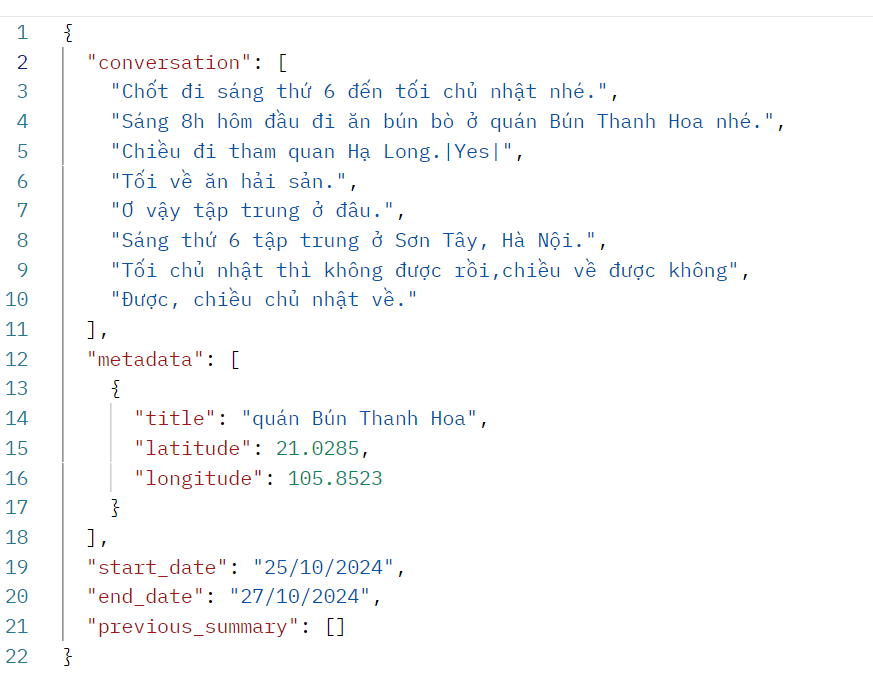
\includegraphics[width=0.8\textwidth]{figures/c4/input.png}
        \caption{JSON request hoàn chỉnh từ client gửi đến server.}
        \label{fig:input}
    \end{figure}

Sau đó, phía server thực hiện xây dựng Prompt. Server FastAPI nhận yêu cầu, tổng hợp dữ liệu và xây dựng một prompt chi tiết cho Google Gemini API (model 2.0 flash), như minh họa trong Hình~\ref{fig:prompt}. Prompt này chứa đầy đủ ngữ cảnh và các chỉ dẫn cụ thể về cách tạo lịch trình dạng JSON theo yêu cầu (lọc sự kiện, xử lý Yes/No, liên kết metadata, gộp lịch trình cũ, tuân thủ định dạng output, v.v.). % (Tham khảo cấu trúc prompt chi tiết tại Phụ lục \ref{apdx:gemini_prompt}) % <<< Placeholder
    \begin{figure}[H]
        \centering
        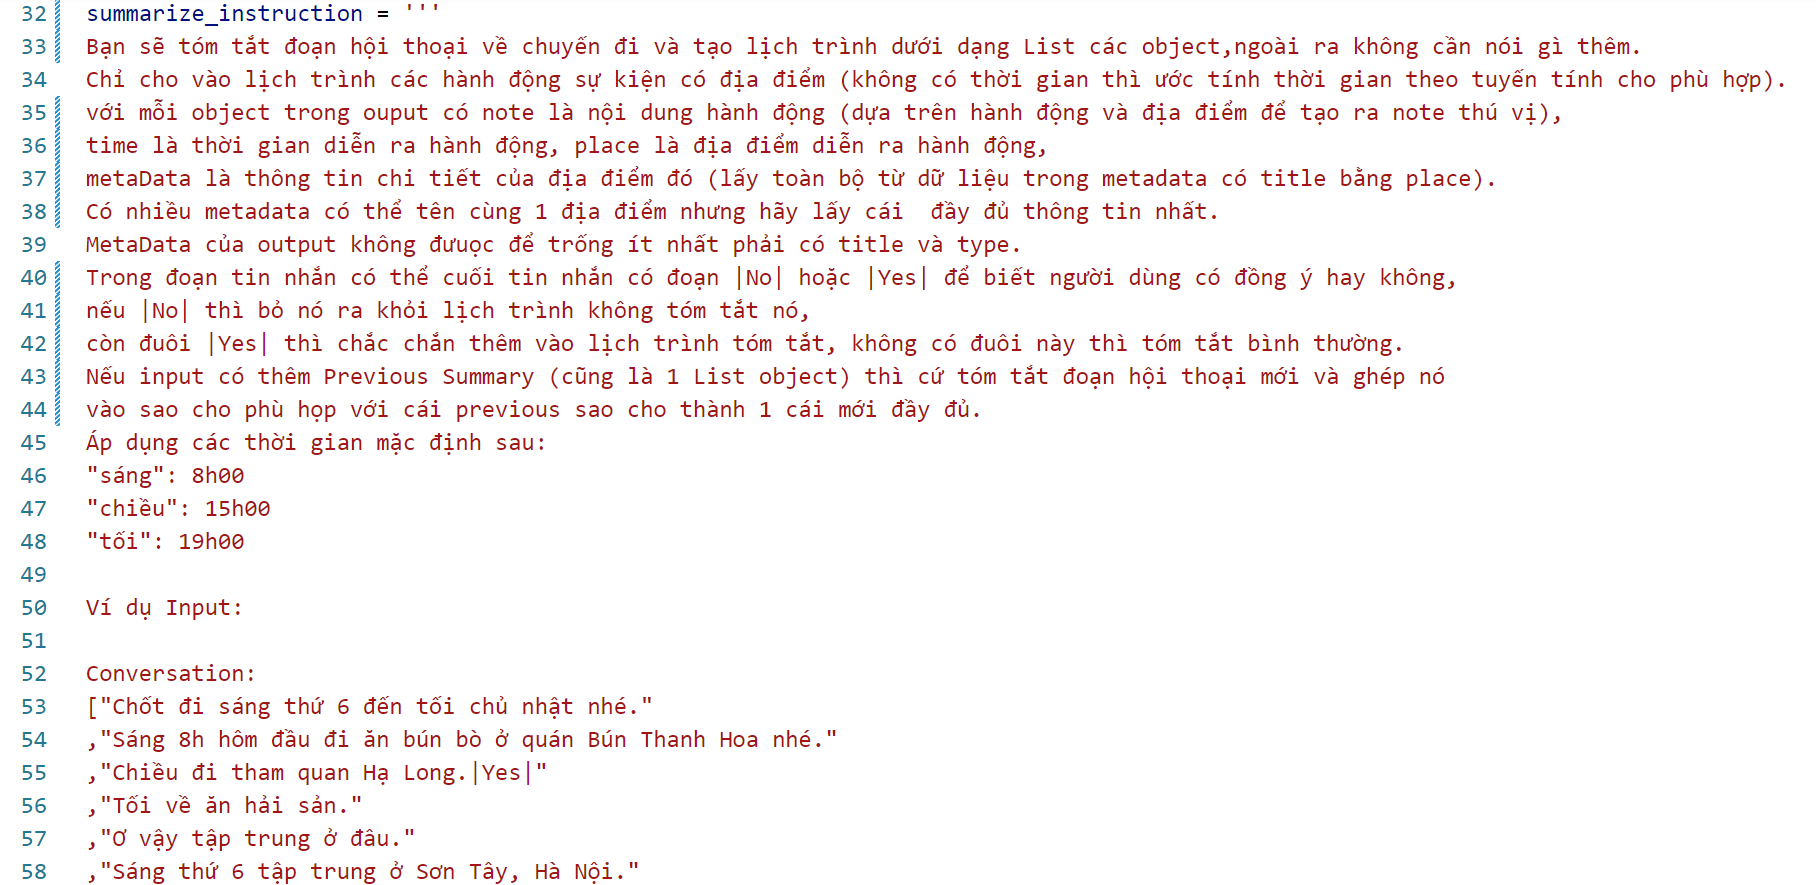
\includegraphics[width=0.9\textwidth]{figures/c4/prompt2.png}
        \caption{Prompt hướng dẫn Gemini tổng hợp lịch trình.}
        \label{fig:prompt}
    \end{figure}

Cuối cùng là bước xử lý kết quả, lưu trữ và phản hồi. Server FastAPI gửi prompt đến Gemini API, nhận phản hồi JSON chứa lịch trình, phân tích cú pháp kết quả đó. Sau đó, server thực hiện thao tác \texttt{upsert} vào bảng \texttt{chat\_summaries} để lưu/cập nhật lịch trình (\texttt{summary}), bản đọc (\texttt{readings}), và \texttt{last\_message\_id}. Kết quả lịch trình cuối cùng (ví dụ như trong Hình~\ref{fig:output}) được gửi về client Flutter để hiển thị.
    \begin{figure}[H]
        \centering
        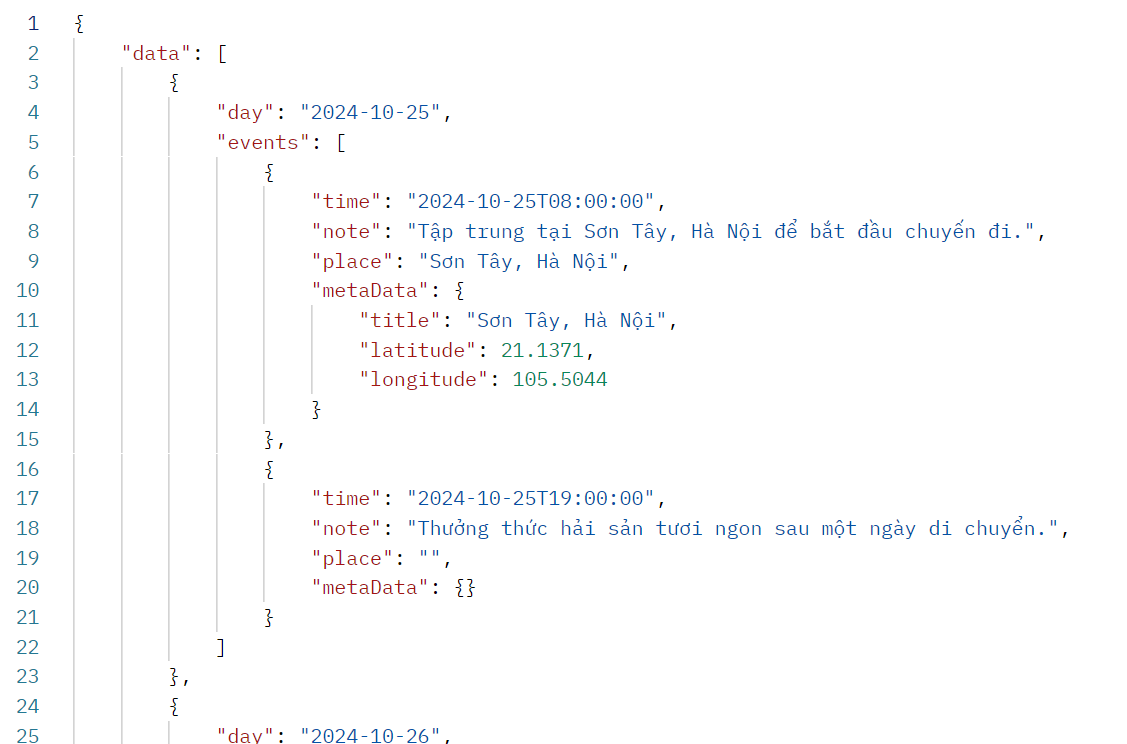
\includegraphics[width=0.8\textwidth]{figures/c4/output.png}
        \caption{Output JSON chứa lịch trình trả về từ server.}
        \label{fig:output}
    \end{figure}

Kiến trúc xử lý hai giai đoạn này, kết hợp tiền xử lý bất đồng bộ và tổng hợp thông minh theo yêu cầu bằng LLM, cho phép VieVu cung cấp tính năng hỗ trợ tạo lịch trình mạnh mẽ và hiệu quả.

